\documentclass[tikz,border=8pt,multi=tikzpicture]{standalone}
\usepackage{amsmath}
\usepackage{xcolor}
\usetikzlibrary{arrows.meta, calc}

\definecolor{mainblue}{HTML}{001158}
\definecolor{accent}{HTML}{8592bc}
\definecolor{lightaccent}{HTML}{e7e9f2}

\tikzset{
  force/.style={-{Stealth[length=3mm]}, line width=1.2pt, color=mainblue},
  dim/.style={-{Stealth[length=2mm]}, line width=0.7pt, color=accent},
  moment/.style={-{Stealth[length=2.5mm]}, line width=1.2pt, color=mainblue},
  every node/.append style={font=\sffamily}
}
\newcommand{\festlager}{
  \draw[line width=1pt] (0,0) -- (-0.3,-0.5) -- (0.3,-0.5) -- cycle;
  \draw[line width=1pt] (-0.42,-0.5) -- (0.42,-0.5);
  \foreach \x in {-0.42,-0.24,...,0.42} {\draw[line width=0.4pt] (\x,-0.5) -- (\x-0.13,-0.68);}
}

\begin{document}

% ---------- Exercise 3.3: cantilever, fixed support, point load ----------
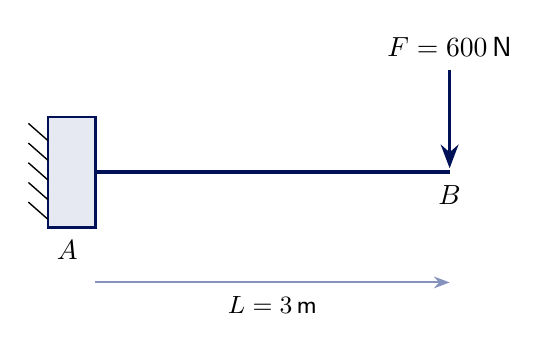
\begin{tikzpicture}
\fill[lightaccent, draw=mainblue, line width=1pt] (-0.6,0.7) rectangle (0,-0.7);
\foreach \y in {-0.6,-0.35,...,0.6} {\draw[line width=0.5pt] (-0.6,\y) -- (-0.85,\y+0.22);}
\draw[line width=1.5pt, mainblue] (0,0) -- (4.5,0);
\node[below left] at (-0.1,-0.75) {$A$};
\node[below] at (4.5,-0.05) {$B$};
\draw[force] (4.5,1.3) -- (4.5,0.05);
\node[above] at (4.5,1.35) {$F=600\,\text{N}$};
\draw[dim] (0,-1.4) -- (4.5,-1.4);
\node[below] at (2.25,-1.45) {\small $L=3\,\text{m}$};
\end{tikzpicture}

% ---------- Exercise 3.4: cantilever, fixed support, inclined load ----------
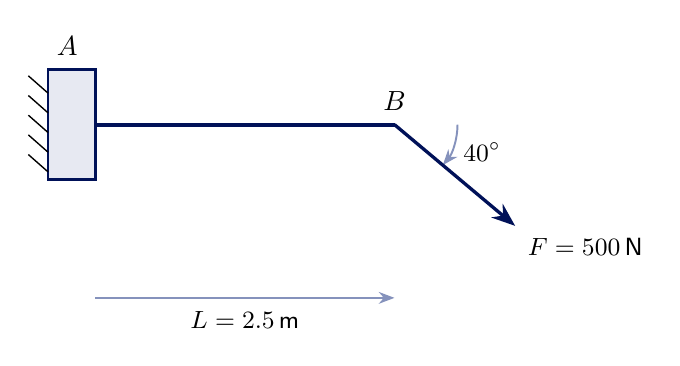
\begin{tikzpicture}
\fill[lightaccent, draw=mainblue, line width=1pt] (-0.6,0.7) rectangle (0,-0.7);
\foreach \y in {-0.6,-0.35,...,0.6} {\draw[line width=0.5pt] (-0.6,\y) -- (-0.85,\y+0.22);}
\draw[line width=1.5pt, mainblue] (0,0) -- (3.8,0);
\node[above left] at (-0.1,0.75) {$A$};
\node[above] at (3.8,0.05) {$B$};
\draw[dim] (4.6,0) arc (0:-40:0.8);
\node[right] at (4.55,-0.35) {\small $40^\circ$};
\draw[force] (3.8,0) -- ++(-40:2.0);
\node[below right] at ($(3.8,0)+(-40:2.05)$) {\small $F=500\,\text{N}$};
\draw[dim] (0,-2.2) -- (3.8,-2.2);
\node[below] at (1.9,-2.25) {\small $L=2.5\,\text{m}$};
\end{tikzpicture}

% ---------- Exercise 3.5: pin support + pendulum-link support ----------
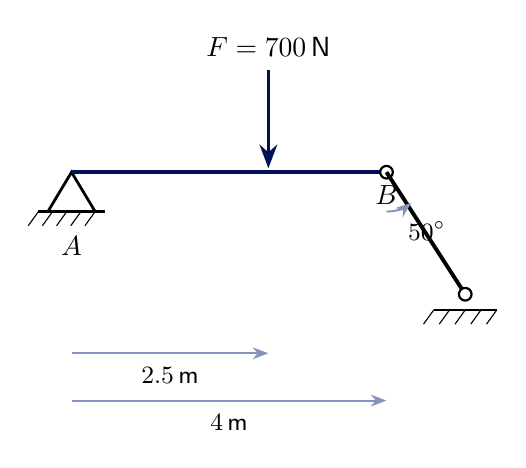
\begin{tikzpicture}
\begin{scope}
  \festlager
\end{scope}
\draw[line width=1.5pt, mainblue] (0,0) -- (4,0);
\node[below] at (0,-0.7) {$A$};
\node[below] at (4,-0.05) {$B$};
\draw[fill=white, line width=0.8pt] (4,0) circle (0.08);
\draw[line width=1.4pt] (4,0) -- (5.0,-1.55);
\draw[fill=white, line width=0.8pt] (5.0,-1.55) circle (0.08);
\draw[line width=1pt] (4.6,-1.75) -- (5.4,-1.75);
\foreach \x in {4.6,4.8,...,5.4} {\draw[line width=0.4pt] (\x,-1.75) -- (\x-0.13,-1.93);}
\draw[dim] (4,-0.5) arc (270:309:0.5);
\node[right] at (4.15,-0.75) {\small $50^\circ$};
\draw[force] (2.5,1.3) -- (2.5,0.05);
\node[above] at (2.5,1.35) {$F=700\,\text{N}$};
\draw[dim] (0,-2.3) -- (2.5,-2.3);
\node[below] at (1.25,-2.35) {\small $2.5\,\text{m}$};
\draw[dim] (0,-2.9) -- (4,-2.9);
\node[below] at (2,-2.95) {\small $4\,\text{m}$};
\end{tikzpicture}

\end{document}
